%%%%%%%%%%%%%%%%%%%%%%%%%%%%%%%%%%%%%%%%%%%%%%%%%%%%%%%%%%%%%%%%%%%%%%%%%%%%%%
%%
%% This file is part of the ASTERICS Framework. 
%%
%% Copyright (C) Hochschule Augsburg, University of Applied Sciences
%% Efficient Embedded Systems Group
%%
%% Author(s): Gundolf Kiefer <gundolf.kiefer@hs-augsburg.de>
%%
%%%%%%%%%%%%%%%%%%%%%%%%%%%%%%%%%%%%%%%%%%%%%%%%%%%%%%%%%%%%%%%%%%%%%%%%%%%%%%



%%%%%%%%%%%%%%%%%%% 2. Using ASTERICS %%%%%%%%%%%%%%%%%%%


\chapter{Using \asterics}\label{ch:02-using} 

\secauthor{Michael Schäferling, Gundolf Kiefer, Philip Manke}


\section{Installation}
\label{sec:02-installation}

Prerequisites for the core parts of \asterics:

\begin{itemize}
\item A Linux based operating system. \asterics is tested for Debian 10
\item We strongly recommend the use of the Bourne-Again-Shell \texttt{bash} for \asterics scripts and Makefiles
\item GNU \texttt{make}
\item Python3, version \texttt{3.5} or higher
\item Python packages: \texttt{numpy} (for generating CNN systems)
\end{itemize}

\asterics-GUI prerequisites:

\begin{itemize}
\item Python packages: \texttt{pyqt5}, \texttt{pandas}.
\item QT5, version \texttt{5.5} or higher
\end{itemize}

Optional prerequisites:

\begin{itemize}
\item Xilinx Vivado 2019.1 (IP-Core packaging and/or synthesizing systems)
\item GraphViz, version \texttt{2.38} or higher (SVG graph generation)
\item Python package \texttt{graphviz}, version \texttt{0.8} or higher (SVG graph generation)
\end{itemize}


The \asterics framework can be used in two ways:

\begin{itemize}
\item As a \textit{portable} installation or
\item as a \textit{fixed} system installation.
\end{itemize}

The \textit{portable} installation is essentially a clone of the \asterics Git repository (Chapter \ref{ch:03-developing}) or an extracted a repository snapshot.
To utilize \asterics in this form, \textit{source} the file \texttt{settings.sh} in the repository's root folder, using:

\begin{lstlisting}[style=shell]
  $ source settings.sh
\end{lstlisting}

\bigskip

The \textit{fixed} installation requires a clone or extracted snapshot of the \asterics Git repository.
To install \asterics to your system, use the provided makefile install target:

\begin{lstlisting}[style=shell]
  $ make install PREFIX=<install path>
\end{lstlisting}

You may need to provide root permissions depending on your installation path.
To now use the installation, you need to source the file \texttt{settings.sh}, as you would for the portable installation.

\begin{lstlisting}[style=shell]
  $ source <install path>/settings.sh
\end{lstlisting}

Optionally, for convenience, we suggest adding an alias for the sourcing command to your \texttt{.bashrc} file.


\section{Getting Started with the Supplied Demo System}
\label{sec:02-getting_started}

The \asterics framework provides at least one demonstration system to get in touch with the concepts of the framework and its modules.
The system may also be used as a basis for further development.

The demo system is equipped with a \texttt{Make} based build system.
With this, a specific \asterics chain is prepared, which is then integrated into the system during the build step.
During the build step, the required embedded software for proper operation is also supplied.
After hardware synthesis and software compilation, the demo system can be put into operation on the specific board.
The system is tested using Vivado versions 2019.1 and 2020.2.


In section \ref{sec:06-02-user_guide} a short user guide describes the necessary steps for building the demo system \texttt{as\_refdesign\_zynq} with a focus on the \asterics system generator \textit{Automatics}.
Here, \textit{Automatics} is described in less detail with more focus on the build process itself.

The following prerequisites are necessary to build and use the demo system:

\begin{itemize}
\item (optional) A hardware target. To run the demo system as is, the Zybo\footnote{\url{https://store.digilentinc.com/zybo-zynq-7000-arm-fpga-soc-trainer-board/}} board and an OmniVision OV7670 camera module are required. Necessary cable drivers and board files need to be installed.
For other hardware targets, the constraint files and the Vivado project (block design) need to be modified manually.
\item (optional) To view the demo system in action, a monitor with a VGA or HDMI input connected to the hardware is required.

\bigskip
\emph{NOTE:} If your Linux distribution does not support the \texttt{source} command by default (Ubuntu, Debian, ...), it does not use \textit{bash} as the standard shell. You need to either modify this setting system-wide or explicitly run each of the files that is passed to the \texttt{source} command in the steps below.


\end{itemize}

Follow the following steps to build the demo system \texttt{"as\_refdesign\_zynq/"}:

\begin{enumerate}

\item Setup and optionally install \asterics. Refer to Section \ref{sec:02-installation} for this step.
\item Source your \asterics installation:
	\begin{lstlisting}[style=Shell]
 > source <asterics root / installation>/settings.sh
  \end{lstlisting}
\item Set up a workspace directory and move into it:
  \begin{lstlisting}[style=Shell]
 > mkdir asterics-workspace && cd asterics-workspace
  \end{lstlisting}
\item Copy the directory \texttt{asterics/systems/as\_refdesign\_zynq/} to your workspace:
  \begin{lstlisting}[style=Shell]
 > cp -a <asterics root / installation>/systems/as_refdesign_zynq/ .
  \end{lstlisting}
\item Optional: If you intent to build the Vivado IP-Core (also needed to build the whole system), you need to source your Vivado installation:
  \begin{lstlisting}[style=Shell]
 > source <VIVADO-DIR>/settings64.sh
  \end{lstlisting}
\item Move into \texttt{as\_refdesign\_zynq/} in your workspace:
  \begin{lstlisting}[style=Shell]
 > cd as_refdesign_zynq
  \end{lstlisting}
\item Now you can build the system. You can generate only the \asterics source files using:
  \begin{lstlisting}[style=Shell]
 > make asterics_core
  \end{lstlisting}
  \textbf{This generates the \asterics hardware (VHDL) and software (C) files for the demo system to \texttt{./asterics\_core}.
  From here you can inspect the files, modify them and/or include them in your projects or FPGA toolchains other than Xilinx Vivado.}

\item If Vivado is available, you can generate Xilinx-specific output products:
	{
    \begin{enumerate}
	\item You can generate the \asterics IP-Core (to be used in a Vivado project) using:
    \begin{lstlisting}[style=Shell]
 > make asterics_vivado_cores
    \end{lstlisting}
    The IP-Core will be generated to the directory \texttt{vivado\_cores}.
    From here you can include this directory into the IP-Catalogue of Vivado.
    Now you can inspect the IP-Core and add it to block designs.
  \item You can build the entire FPGA project (after the Vivado IP-Core was generated, see above), using:
    \begin{lstlisting}[style=Shell]
 > make build_system
    \end{lstlisting}
  Note that this will take some time, depending on the capabilities of your development system.
  This creates and builds a full Vivado project with a block design targeting the ZYBO board.
  After synthesis and implementation you can open the project in the GUI using:
  \begin{lstlisting}[style=Shell]
 > vivado hardware/build/system.xpr
  \end{lstlisting}
  \item If you have a ZYBO board and OV7670 image sensor board handy, you can program the hardware and software onto the target boards FPGA by running:
    \begin{lstlisting}[style=Shell]
 > make run
    \end{lstlisting}
  \item Alternatively: To build, implement and compile the hardware and software and flash it onto the board in one step, you can execute:
    \begin{lstlisting}[style=Shell]
 > make build_and_run
    \end{lstlisting}
  or
    \begin{lstlisting}[style=Shell]
 > make all
    \end{lstlisting}
	\end{enumerate}
	}
\end{enumerate}


\section{Getting Started with the \asterics GUI}

\infobox{The \asterics-GUI is still in development and not fully tested. See the application and this documentation as in-flux and experimental.}

The \asterics framework provides a Graphical User Interface (GUI), which is currently under development, with some basic features already available.
Currently, the GUI provides a module browser with information about all modules that come with \asterics and a wizard for setting up Automatics scripts for demo systems and simple systems from scratch.

For more information on the \asterics-GUI and for a user guide, see Section \ref{ch:06-05-tools-gui}.


\section{How to Design \asterics Systems}
\secauthor{Philip Manke}

The \asterics system generator tool \textit{Automatics} automates most of the process of generating an \asterics system and packaging it into an IP-Core and is the official way to create \asterics systems.

\subsection{Design Flow Overview and Terminology}

To start working with \asterics, first an \asterics installation must be procured.
For instructions refer to section \ref{sec:02-installation}.


Generally, we recommend using a Linux based operating system for working with \asterics, as most tools are used on the command line and Makefiles are supplied to automate portions of the process of building \asterics systems.
Furthermore, MAC OS and Microsoft Windows have not been tested.

\subsubsection*{Terminology}

\begin{itemize}
\item \textbf{\asterics:} The entire framework. This includes everything within the git repository.
\item \textbf{\asterics Installation:} A local copy of the \asterics git repository at a known location.
\item \textbf{\asterics Settings File:} A short script that is used to set certain environment variables required by some tools to function correctly and be available from the command line. Used best with the \texttt{source} command.
\item \textbf{IP-Core:} An Intellectual Property - Core (IP-Core) is a packaged hardware and software subsystem for integration into a larger system.
\item \textbf{Hardware Module:} A module with purely hardware source files. 
\item \textbf{Software Module:} A module with purely software source files.
\item \textbf{\asterics Module:} A hardware and / or software module included with \asterics. These modules are manually developed and provide common functionality. They may describe image processing operations, common data management tasks, infrastructure or support other modules similar to a library. They are contained in the \texttt{modules} folder.
\item \textbf{Module Repository:} A directory containing \asterics modules using the file structure laid out in section \ref{sec:02-file_structure}.
\item \textbf{\asterics Chain / \asterics System / \asterics IP-Core:} A specific configuration built from \asterics modules, comprising both hardware and software.
It must be integrated into a larger system to be synthesized and programmed onto an actual hardware target.
These terms are often used interchangeably, though generally \asterics chain specifically refers to the concept of the \asterics subsystem of modules, \asterics system may also refer to a larger system that has an \asterics chain integrated into it and \asterics IP-Core may refer specifically to an \asterics chain that was packaged to an IP-Core to be integrated into a larger system.
\item \textbf{Generic:} A configuration parameter for an \asterics module. This name comes from the hardware description language VHDL, that all modules are written in.
\item \textbf{Port:} A single input or output for data or control signals of a hardware module.
\item \textbf{Interface:} A standardized arrangement of ports. The name, data type, direction and function of each port is defined.
\item \textbf{Automatics:} The \asterics system generator tool.
\item \textbf{Chain Description Script:} Build instructions for Automatics in Python syntax to build an \asterics chain.
\item \textbf{Module Specification Script:} A small Python script providing meta-information for each \asterics module.
Automatics requires this script to analyse an \asterics module - one script per module.
\item \textbf{2D Window Pipeline:} A hardware architecture for the efficient implementation of sliding window buffers, required by systems with multiple window modules.
\item \textbf{Window Module / Filter Module}: An \asterics module for use within a 2D Window Pipeline.
This kind of module has a special input port to receive multiple pixels from different locations in the image simultaneously.
\end{itemize}

\subsubsection*{\asterics Design Flow}
The following list describes the broad steps of the typical design flow for \asterics systems:

\begin{enumerate}
\item The process of using \asterics always begins with sourcing the \asterics settings file, as described in section \ref{sec:02-getting_started}.
\item We recommend to start the command line interface (CLI) or the graphical version (GUI) of the \asterics module browser to get an overview of available \asterics module, their interfaces, ports and configuration generics.
Using the tools, \asterics modules for use in the processing chain and functionalities that may require new modules are identified.
\item To get started quickly, we recommend to copy an existing system from \texttt{asterics/systems/}.
At least a new (blank) chain description script for the \asterics chain and any hardware specific files, such as constraint files, are required.
\item To describe your system using Automatics, the chain description script must be edited.
In the example system it can be found in \lsthdlinline{as\_refdesign\_zybo/asterics/image\_differencing/asterics-gen.py}
\item Using a module browser (GUI or CLI) to identify the names of the desired modules they are added to the chain description, configured and connected with each other.
\item If hardware modules not provided by \asterics are to be used:
	\begin{enumerate}
	\item The module source files are organized in a separate module repository, according to the file structure laid out in section \ref{sec:02-file_structure}.
	\item A module specification script is created for the module detailed in section \ref{sec:06-02-new_modules}.
	\item The module browser is used to analyze the modules by adding the module repository.
	The modules are inspected to make sure they were analyzed correctly.
	\item The module repository import is added to the chain description script.
	\end{enumerate}
\item Desired output products are added to the chain description script and Automatics is run.
\item The generated hardware files may be inspected for any errors.
\item If the Xilinx toolchain is used, Automatics can automatically package the \asterics chain as a Vivado-compatible IP-Core, otherwise the resulting hardware and software files have to be packaged manually.
\item The \asterics IP-Core is integrated into the larger system. \asterics provides AXI slave and master ports for communication.
\end{enumerate}

These major steps are described in detail in the following subsections.


\subsection{Settings up a new Project with Automatics}
\label{ssec:02-setup}

This section details the typical steps necessary to set up a new project using Automatics.


\subsubsection{Setup Steps:}

\begin{enumerate}
\item Install \asterics. See Section \ref{sec:02-installation}.
\item Open a command line interface (preferably using \texttt{bash})
\item Source the \asterics settings file in the installation directory using:
\begin{lstlisting}[style=Shell]
 > source <path to installation>/settings.sh
\end{lstlisting}
\item Create a new project directory and change into it:
\begin{lstlisting}[style=Shell]
 > mkdir <new project system name>
 > cd <new project system name>
\end{lstlisting}
\item Create a new chain description script:
\begin{lstlisting}[style=Shell]
 > touch asterics-gen.py
\end{lstlisting}
\item Open the chain description script in your editor of choice.
We recommend a Python-capable IDE, with the Automatics source files added to the list of auto-complete sources for the best experience.
\end{enumerate}

The entire \asterics chain will now be described in the chain description script using Python commands.
Using Automatics with this description, all necessary hardware files implementing the described chain will be generated and all module source files necessary to implement and use the chain will be collected.

To get started with the chain description script, the following two lines need to be added:
\begin{lstlisting}[style=AutomaticsPython]
 import asterics
 chain = asterics.new_chain()
\end{lstlisting}

The first line imports the \lstapyinline{asterics} Python module.
This makes the highest level functions of Automatics available in the rest of the file.
The second line makes use of the \lstapyinline{asterics} Python module, creating a new \lstapyinline{chain}.
Writing \lstapyinline{chain} to the left of the equals sign, assigns the newly created chain to the keyword (variable) \lstapyinline{chain}.
Using \lstapyinline{chain}, the rest of the \asterics chain can now be described.

\subsubsection{Configuring Automatics for the Hardware Target}
\label{ssec:02-hwtargetconfig}

By default Automatics is configured to generate IP-Cores compatible with ZYNQ-7000 series FPGA-SoCs by Xilinx, specifically, the ZYBO development board by Digilent Inc is used as the reference board.

Certain parameters have to be explicitly provided in the chain description script to target a different FPGA.

The following commands are provided by Automatics:\\
\begin{itemize}
\item \lstapyinline{chain.define_hardware_target("partname", "design name", "board")}\\
This command defines which FPGA part the generated IP-Core is compatible with (\texttt{"partname"}), the internal name of the packaged IP-Core (\texttt{"design name"}) and the specific FPGA board it is packaged for (\texttt{"board"}).
These parameters only apply to automatic IP-Core packaging using Automatics and Xilinx Vivado.
\item \lstapyinline{chain.set_ipcore_name("name", "description")}\\
This command sets display name of the packaged IP-Core (\texttt{"name"}) and its description (\texttt{"description"}).
These values will be visible in the IP Repository of Xilinx Vivado.
These parameters only apply to automatic IP-Core packaging using Automatics and Xilinx Vivado.
\item \lstapyinline{chain.set_asterics_base_address(<address>, <address space size>)}\\
This command changes the base address and optionally the size of the address space for the \asterics IP-Core.
The base address is required as the slave register manager of \asterics requires to know the base address in order to decode them.
The address space size has no impact on the hardware generated.
Automatics uses it to warn the user if too many registers are present in an \asterics chain, not mappable to the register address space.
\end{itemize}

\subsection{Adding Modules to the \asterics Chain}
\label{ssec:02-adding}

An \asterics chain consists of \asterics modules that each fulfill cohesive tasks to comprise a complete image, video or general data processing system.
Modules may have tasks such as data management, general infrastructure, image processing, general processing, etc.

The \asterics installation provides a collection of modules, free to use.
To browse the available modules in a graphical user interface using QT5, use:
\begin{lstlisting}[style=Shell]
 > as-module-browser
\end{lstlisting} 

Alternatively, a command line interface is available with:
\begin{lstlisting}[style=Shell]
 > as-module-browser-cli
\end{lstlisting}

Once a desired module is determined, it can be added to the \asterics chain using the following command:
\begin{lstlisting}[style=AutomaticsPython]
module = chain.add_module("entity name")
\end{lstlisting} 

To tell Automatics which module should be added to the chain, provide the entity name of the module to the command \lstapyinline{add_module}.
Both the CLI and GUI module browser list this name for each module.
As with the chain object, the newly added module is also assigned to a new keyword, so it can be referenced later in the chain description script.
Use a short but memorable and easily identifiable name for each module you add to the chain, for example:
\begin{lstlisting}[style=AutomaticsPython]
result_writer = chain.add_module("as_memory_writer")
\end{lstlisting}

Additionally, two further parameters can be provided to the command \lstapyinline{add_module}:

The second parameter, \texttt{user name}, will optionally name the hardware module instantiated in the generated files.
Signals that connect from the module will also be generated with the provided name included, making the generated code easier to read and especially making it easier to distinguish external interfaces of the resulting IP-Core.

The third parameter, \texttt{repo\_name}, optionally defines from which module repository the requested module should be selected.
It is only necessary to define the repository, if two modules with the same \texttt{entity name} exist, for example, if a modified version of a standard \asterics module exists.

The \lstapyinline{add_module} command with all three parameters may look like this:
\begin{lstlisting}[style=AutomaticsPython]
camera = chain.add_module("as_sensor_ov7670", "cam0", "default")
\end{lstlisting}

If custom modules are to be used with Automatics, they first have to be imported.
To import new modules to Automatics, the following command is used in the chain description script:
\begin{lstlisting}[style=AutomaticsPython]
asterics.add_module_repository("path", "repository name")
\end{lstlisting}
The parameter \texttt{"path"} of the command tells Automatics, where to look for new modules.
The path to a directory that is organized in the same way as the \texttt{modules} directory of \asterics, as described in section \ref{sec:02-file_structure}, should be provided.
The parameter \texttt{"repository name"} is optional and can be set to any name desired.
It may prove useful to differentiate between multiple imported module repositories, as specific repository can be defined when using the \lstapyinline{add_module()} command is used.
The command can be used at any point after \lstapyinline{import asterics} in the chain description script, however, we recommend putting it before the command creating a new chain.

\subsection{Configuring \asterics Modules}
\label{ssec:02-configuring}

This section gives a basic overview of the most common configuration options for \asterics modules.
Section \ref{ssec:02-example-script} provides a short example script with valid configuration commands.

\subsubsection{Configuring Module Parameters: Generics}

Modules added to the chain can be configured with their own parameters, using \textit{Generics}.
Each module has a different set of generics, most with default values, if they are not explicitly assigned a value in the chain description script.

The generics and their default values of a module are available using a module browser or by directly consulting the source code of the module.
The effect of each generic is currently only explained either in the source code of the module of in the reference of the module in this manual.

Assigning a new value to the generic is done using the following command:
\begin{lstlisting}[style=AutomaticsPython]
module.set_generic_value("GENERIC NAME", "value")
\end{lstlisting}

To tell Automatics which generic to modify, the \texttt{GENERIC NAME} specifies the generic using its name as it appears in the source code.
The module browsers list the generic's names for all modules.

The \texttt{value} is what the generic will be assigned.
This parameter can be any number (integer or float) or string.

\emph{Note:}
The value provided for the \texttt{value} parameter will be directly written into the generated source code.
For example: To set the generic \texttt{KERNEL\_TYPE} of the module \texttt{conv\_filter} to \lsthdlinline{"laplace"}, the following command has to be used:
\begin{lstlisting}[style=AutomaticsPython]
conv_filter.set_generic_value("KERNEL_TYPE", '"laplace"')
\end{lstlisting}

Note how the double quotes of the value \lsthdlinline{"laplace"} are only carried over to generated VHDL code if they are inside a string themself, by using single quotes to encompass the entire value.
The same can be achieved using triple double quotes: \lstapyinline{""" "laplace" """} or by escaping the double quotes: \lstapyinline{"\\"laplace\\""}.
Similarly, for \lsthdlinline{std_logic} values, delimited in VHDL by single quotes, these have to be encased in double quotes in the chain description script, for example:
\begin{lstlisting}[style=AutomaticsPython]
module.set_generic_value("EXAMPLE_GENERIC", "'0'")
\end{lstlisting}

\subsubsection{Configuring Module Ports}

For some ports of modules you may want to assign a static value, for example if the functionality of the port is not used in the specific chain that is described.
By default Automatics will assign a \textit{neutral value} to ports that are left unconnected.
This value depends on the data type and direction of the port, for further details, refer to section \ref{sec:06-02-default}.
To assign a static value to a port, use the following command:
\begin{lstlisting}[style=AutomaticsPython]
module.set_port_fixed_value("port name", value)
\end{lstlisting}
To tell Automatics which port should be modified, the name of the port must be provided as the first parameter to this command.
To assure that the correct port is selected, the full name of the port should ideally be provided.
As with assigning values to generics, the value of the parameter \texttt{value} will be directly inserted into the generated VHDL code and must therefore follow VHDL syntax.
The following are examples for the correct use of the command:
\begin{lstlisting}[style=AutomaticsPython]
result_writer.set_port_fixed_value("mem_req_ack", "'1'")
image_reader.set_port_fixed_value("stall_out", "open")
edge_filter.set_port_fixed_value("threshold", 'X"C418"')
inverter.set_port_fixed_value("data_in", "s_camera_data(7 downto 0)")
\end{lstlisting}

Furthermore, ports may also be configured to face the outside of the entire \asterics chain.
For example, if an external device, such as a video camera, is to be connected to the \asterics chain, the module that should be connected to the device needs to provide the necessary ports for it.
These ports must be available as ports of the \asterics IP-Core, at the highest level of the chain, or \textit{external}.
For this and similar purposes, ports can be \textit{made external} using the following command:
\begin{lstlisting}[style=AutomaticsPython]
module.make_port_external("port name", value)
\end{lstlisting}
To tell Automatics which port of the module to modify, the port's name must be provided as the first parameter for this command.
The second parameter is optional and by default is taken to be set to \lstapyinline{True}.
If set to \lstapyinline{True}, the command will make the port external.
If set to \lstapyinline{False}, the command can make reverse the effect of making a port external.
Some ports are set to be external by default, this command can make these ports "internal" again.
The following are examples for the correct use of the command:
\begin{lstlisting}[style=AutomaticsPython]
result_writer.make_port_external("flush")
camera.make_port_external("data_in", True)
image_reader.make_port_external("flush_in", False)
\end{lstlisting}

\subsubsection{Configuring Module Interfaces}

An interface of an \asterics module is a collection of ports.
As with ports, an entire interface may also be configured to face the outside of the \asterics chain to be connected with other IP-Cores or external devices later.
For this a similar command is available:
\begin{lstlisting}[style=AutomaticsPython]
module.make_interface_external("interface name", "direction",
                               "interface type", value)
\end{lstlisting}
To tell Automatics which interface to modify, the first three parameters are used to provide identifying information about the interface.
The interface's name suffices in many cases, which is why the other parameters are optional.
If the name is ambiguous, the interface's direction and type should be provided to uniquely identify the desired interface.
The parameter \texttt{value} can be used to invert the functionality of this command, making already external interfaces internal, by setting the parameter to \lstapyinline{False}.

\subsection{Describing Connections}
\label{ssec:02-connecting}

\asterics chains process data that flows through the system in a way akin to a pipeline.
Data is passed from module to module, being processed each step of the way.
In Automatics, the connections are handled in a per-port manner, each port is connected individually.
However, not every connection of every port has to be explicitly described.
Section \ref{ssec:02-example-script} provides a short example script with valid connection commands.

\subsubsection{Connection Commands}

Automatics provides the following ways to connect ports, entire interfaces and entire modules with each other:\\
\begin{itemize}
\item \lstapyinline{module0.connect(module1)}\\
The most general way to describe a connection.
For all unconnected source ports and source interfaces of \lstapyinline{module0} a connection with any matching sink port and sink interface of \lstapyinline{module1} is attempted.
Automatics has several built-in checks to prevent connections between incompatible ports.
For example, the port direction and the data type are checked before a connection is committed.
Similarly, for interfaces, their direction and interface types are also checked to match.
Modules must always be connected in the direction of data flow:
The data source module must be to the left of the \lstapyinline{connect()} command, the data sink module within the parenthesis of the \lstapyinline{connect()} command.
\item \lstapyinline{module0.get_interface("interface name").connect(module1)}\\
To more precisely describe a connection of an interface, the command \lstapyinline{module.get_interface("interface name", "direction", "interface type")} can be used.
The second and third parameters are optional and only required if the interface name alone would be ambiguous.
Use a module browser to find interface names, directions and types of modules.
The \lstapyinline{get_interface()} command followed by \lstapyinline{connect()} tells Automatics to apply the connection only to the interface specified.
If an entire module is provided for the connection target, Automatics will connect the interface to the first matching interface that is found in the module.
\item \lstapyinline{module0.get_port("port name").connect(module1)}\\
To define a single port that should be connected, the \lstapyinline{get_port("port name")} command can be used.
Use a module browser to find the port names of modules.
This command followed by the \lstapyinline{connect()} command tells Automatics to apply the connection only to the port specified.
If an entire module is specified, Automatics will connect the port to the first matching port of the target module.
\item \lstapyinline{module0.get_interface("interface name").connect(module1.get_interface("interface name"))}\\
For precise interface to interface connections, an interface can be provided to the \lstapyinline{connect()} as well.
In this case, Automatics will only attempt a connection between the specified interface of \lstapyinline{module0} and the specified interface of \lstapyinline{module1}.
For example, the following command will connect the output interface of \lstapyinline{camera} with the input of \lstapyinline{writer}:\\
\lstapyinline{camera.get_interface("out").connect(writer.get_interface("in"))}
\item \lstapyinline{module0.get_port("port name").connect(module1.get_interface("interface name"))}\\
This command causes Automatics to attempt connections between the port specified of \lstapyinline{module0} and the ports of the interface specified of \lstapyinline{module1}.
The port will be connected to the first matching port of the interface.
\item \lstapyinline{module0.get_port("port name").connect(module1.get_port("port name"))}\\
This command is the most precise connection command, specifying only a source and target port, therefore only a single connection is attempted.
This command is special, as an important check of the connection process is skipped.
Specifically, the check for equality of the ports' names, allowing the connection between two ports with different names. 
\end{itemize}

\subsubsection{Recommendations and General Rules}

The following list contains general rules and recommendations that apply to the \lstapyinline{connect()} command:

\begin{itemize}
\item Connections to multiple targets, from a port or interface with the direction \lstapyinline{"out"} to ports or interfaces with the direction \lstapyinline{"in"}, are possible by simply using the two necessary connect commands.
Connections from multiple sources to the same target are not allowed as they would in most cases result in problems when synthesizing the resulting hardware description.
\item The \lstapyinline{connect()} command is mostly direction agnostic.
Except when specifying an entire module, the interfaces and ports provided will be internally sorted into source and sink.
However, to be more consistent and readable in the chain description script, we strongly recommend to always write the data source, direction \texttt{out}, to the left of the \lstapyinline{connect()} command and the data sink, direction \texttt{in}, within the parentheses of the \lstapyinline{connect()} command.
\item We recommend to use the commands \lstapyinline{get_interface()} and \lstapyinline{get_port()} especially for modules with many ports and or interfaces.
For simple modules the short-hand command \lstapyinline{get()} generally suffices.
\lstapyinline{get("name", "direction", "interface type")} is a combination of the interface and port specification commands, first searching for an interface of the provided name and then for ports.
As it is possible that a port and interface have the same name, using this method is only recommended when used with simple modules or by more experienced users of Automatics.
\end{itemize}

\subsubsection{Example Chain Description Script}
\label{ssec:02-example-script}

For complete example chain description scripts, refer to section \ref{sec:06-02-user_guide} and the reference designs provided with \asterics in \texttt{asterics/systems/}.

The following are examples for the correct usage of the \lstapyinline{connect()} command in the context of an example chain description script:
\begin{lstlisting}[style=AutomaticsPython]
# Setup:
import asterics
chain = asterics.new_chain()

# Add modules to the chain:
camera = chain.add_module("as_sensor_ov7670")
collect = chain.add_module("as_collect")
writer = chain.add_module("as_memwriter")

# Configuration examples using the writer module:
# Define generic values
writer.set_generic_value("DIN_WIDTH", 32)
writer.set_generic_value("MEMORY_DATA_WIDTH", 32)
# Configure "flush_in" port: 
# Make it available in the interface of the IP-Core
writer.make_port_external("flush_in")

# Connection examples
# Connecting camera and collect (interfaces of type "as_stream"):
camera.connect(collect)
# or
camera.get_interface("out").connect(collect)
# or
camera.get("out", "out", "as_stream").connect(
    collect.get("in", "in", "as_stream")
)
# or
camera.get_port("data_out").connect(collect.get_port("data_in"))
camera.get_port("strobe_out").connect(collect.get_port("strobe_in"))
# ...
camera.get_port("vsync_out").connect(collect.get_port("vsync_in"))

# Connecting collect with writer
# Valid
collect.connect(writer)
# Incorrect, not consistent with the direction of data flow
writer.connect(collect)
# Valid, data flow restriction only applies to modules,
#    not interfaces and ports
writer.get_interface("in").connect(collect.get_interface("out"))
\end{lstlisting}


\subsection{2D Window Pipeline Subsystems}
\label{ssec:02-2dwpl}

This section first provides a brief explanation of the concept of 2D Window Pipeline architectures,  followed by the steps required to describe a 2D Window pipeline implementation using Automatics.
The makeup of window modules and difference to regular \asterics modules will also be touched upon.

\subsubsection{What is a 2D Window Pipeline?}

In a nutshell: The 2D Window Pipeline is a hardware architecture for the efficient implementation multiple sliding window buffers.

\subsubsection{Sliding Window Buffers}

A sliding window buffer is required for processing modules that need access to multiple pixels of the input image at once.
This includes modules that implement image convolution with a kernel, such as Gauss, Sobel and Laplace filters, as well as morphological operations, such as opening and closing and comparison operations such as non-maximum-suppression.

\begin{figure}[htb]
\centering
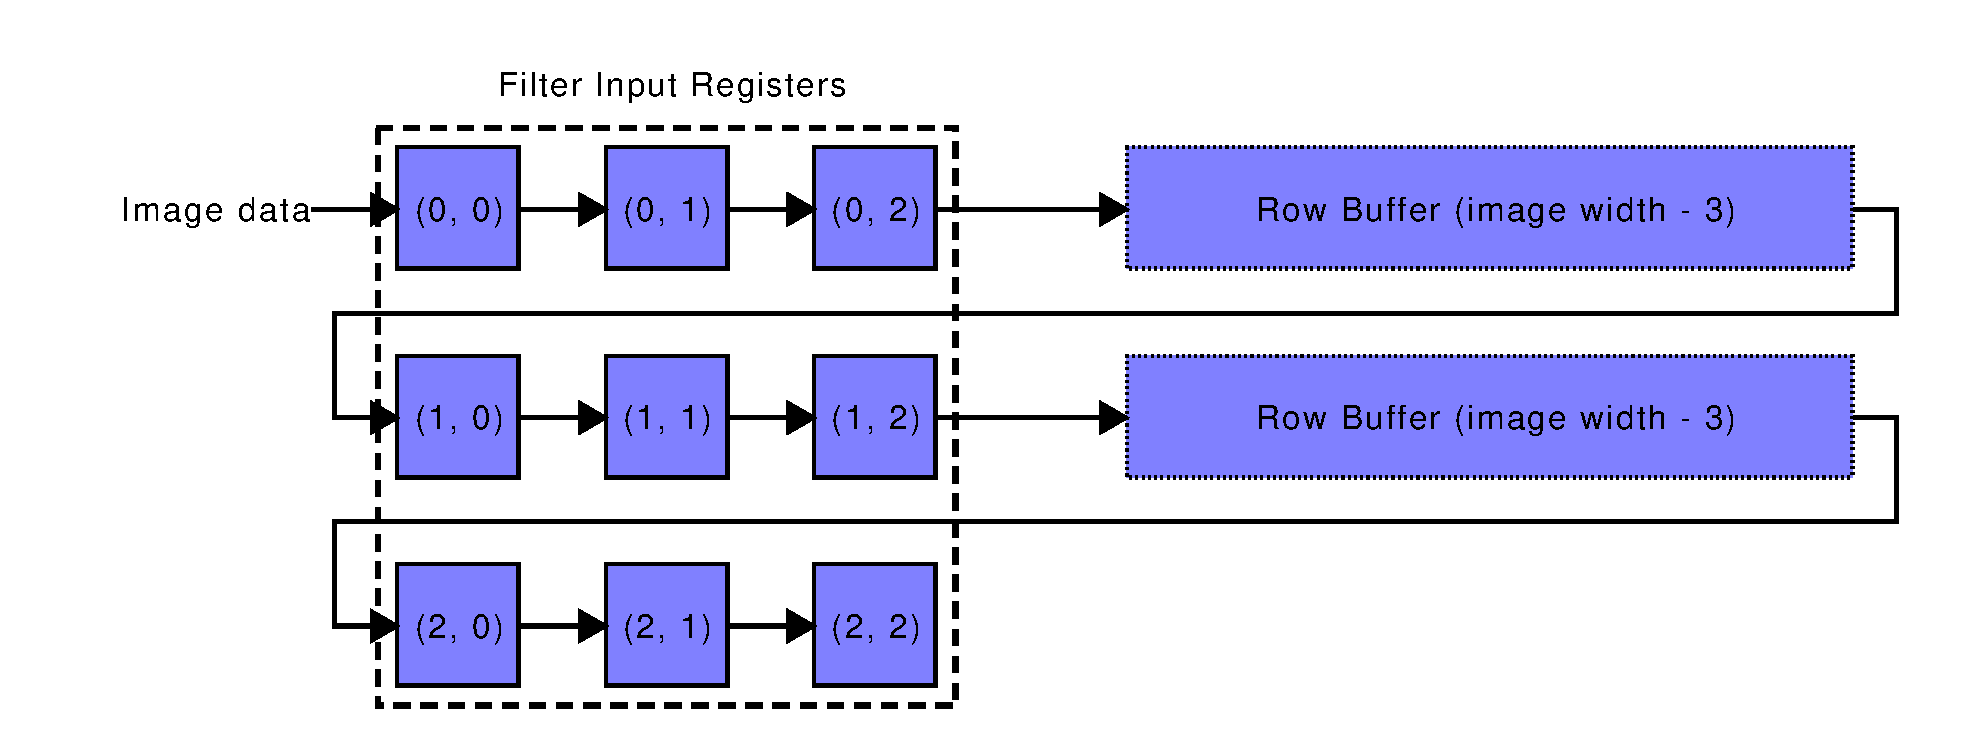
\includegraphics[width=\textwidth]{figs/02-window_buffers_visual.pdf}
\caption{Representation of a sliding window buffer with window size 3 by 3.}
\label{fig:02-sliding_window_buffer}
\end{figure}

Figure \ref{fig:02-sliding_window_buffer} shows a representation of a sliding window buffer as it may be implemented in hardware.
The small cubes represent the hardware registers required to store a single pixel of the image.
Each register contains the relative pixel coordinates.
As the image processing module must have direct and simultaneous access to all pixels in the \textbf{Filter Window}, registers \textit{have} to be used to store those pixels.
The \textbf{Row Buffer}s each store the remaining pixels of a single image row.
For the window size of 3 by 3, as shown in the figure, two complete rows of the image, plus three pixels have to be stored in hardware to implement immediate access to all pixels used by the filter.
This \textbf{sliding window buffer} effectively implements a hardware component that provides a small section of the image to the processing module, the filter window.
By feeding a pixel stream into the buffer, the section moves across the image one pixel at a time for every pixel inserted into the buffer.
The row buffers effectively delay the pixels that are input to them, so they line up with the other pixels within the filter window.
This means that, per pixel input to the sliding window buffer, only one pixel is read from the row buffer  and only one pixel is written to the buffer.
Thus, more efficient memory components, such as block RAM, can be used to implement the buffers.

\subsubsection{2D Window Pipelines}

Oftentimes, image processing systems require multiple filter operations that each require access of multiple pixels simultaneously, for example the Canny edge detector.
In the case of a simple implementation of a Canny edge detector, five processing modules require filter windows of various sizes.
Most modules require a window of the image after it was processed by a previous filter module in the image processing chain.
For these kind of systems, the 2D Window Pipeline architecture can optimize the row buffers required for all of the sliding window buffers.
By merging the row buffers and using block RAM memory components to store large amounts of pixel data, the 2D Window Pipeline can substantially reduce the amount of hardware resources required by the sliding window buffers.

\begin{figure}[htbp]
\centering
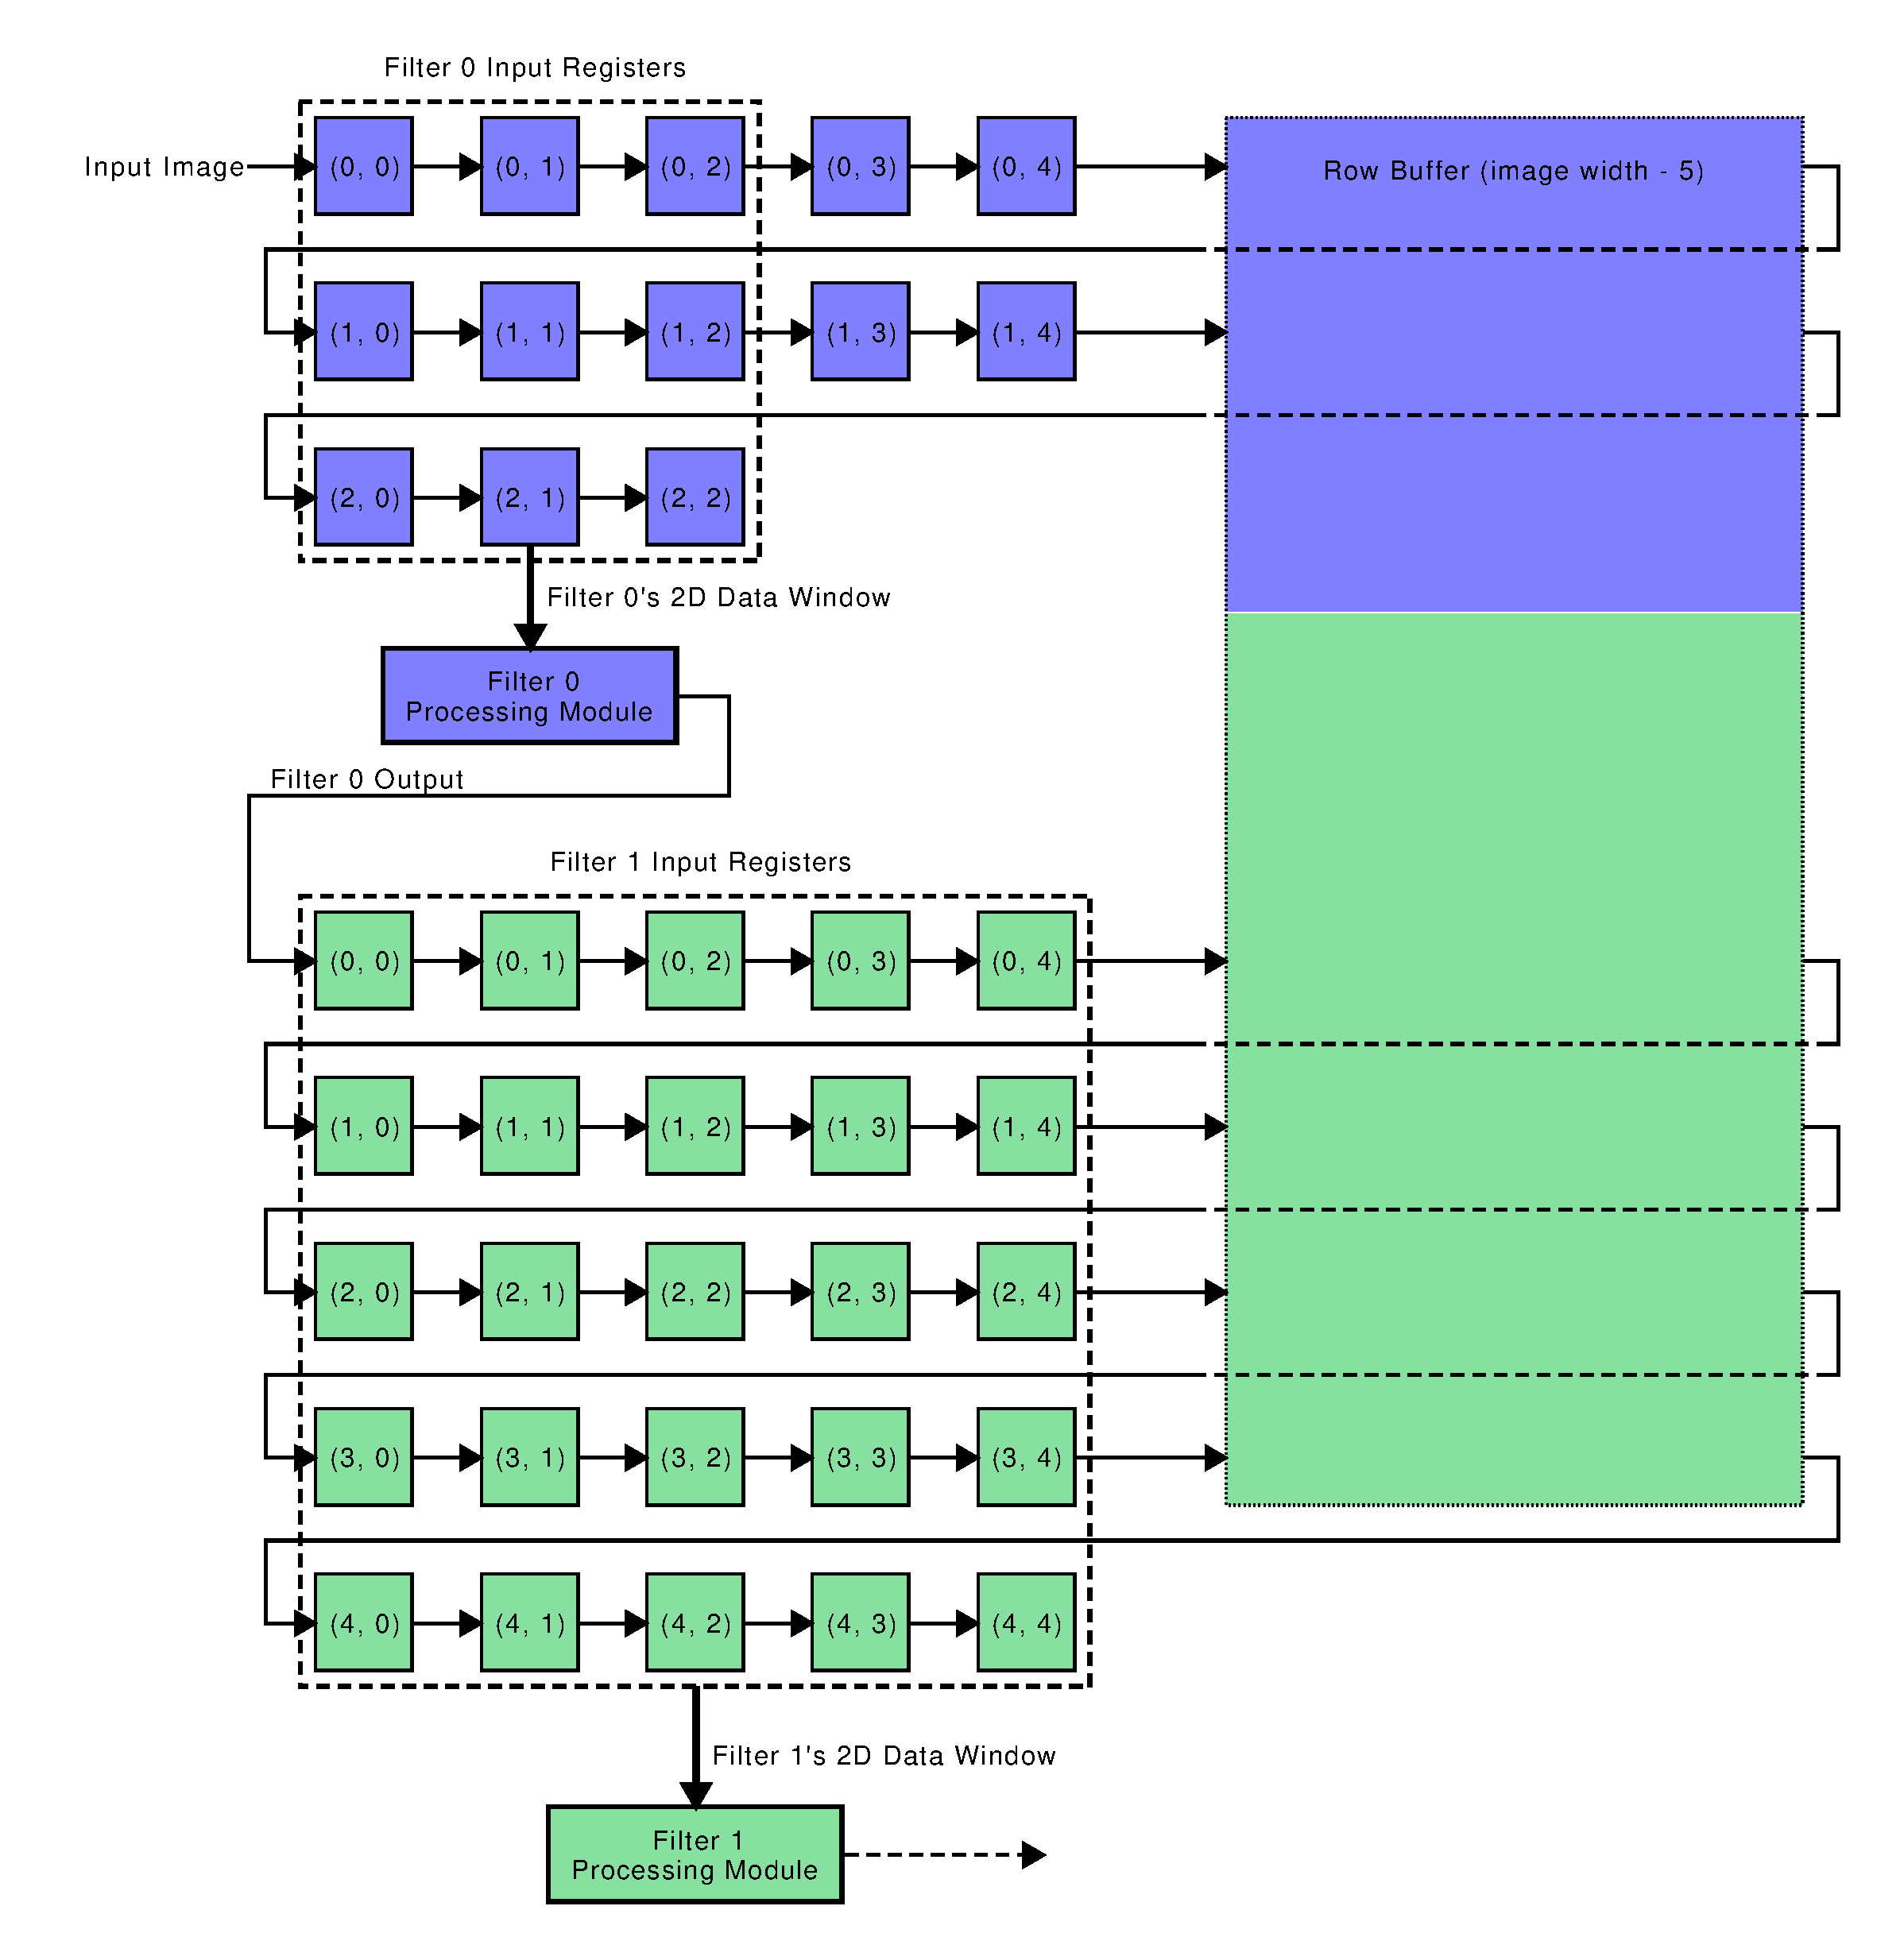
\includegraphics[width=\textwidth]{figs/02-window_buffers_opt_visual.pdf}
\caption{Two sliding window buffers optimized in the 2D Window Pipeline architecture.}
\label{fig:02-buffers_optimized}
\end{figure}

Figure \ref{fig:02-buffers_optimized} shows how two sliding window buffers for filter modules with differing window sizes can be optimized in the 2D Window Pipeline architecture.
All row buffers are merged into a single block RAM component which the synthesis toolchain can further optimize.
The filter window, implemented using registers, is extended for the smaller filter, to enable the merging of all row buffers in this case.
Using different optimization strategies available in the system generator Automatics, the optimizations automatically applied to the pipeline can be configured.


\subsubsection{2D Window Pipelines with Automatics}

Automatics can generate the hardware description code for a 2D Window Pipeline subsystem integrated into an \asterics chain.
Within the pipeline, all data signals that are part of sliding window buffers and all input signals of filter modules are analysed and tagged with delay information.
This data on pixel delays is used to automatically generate a flushing management component used to flush the pipeline when the last image data is to be extracted from it.
Further, delay information is used to generate buffers to synchronize data signals with the main image data stream that is input into the pipeline.
The placement and generation of all sliding window buffer components is fully automatic.

Some of the features of automatically generated 2D Window Pipeline systems include:
\begin{itemize}
\item Fully automatic buffer generation and optimization.
\item Configurable buffer optimization strategies.
\item Arbitrarily shaped filter windows are supported.
\item Automatic generation of synchronization buffers for input signals.
\end{itemize}

Some limitations apply to automatically generated 2D Window Pipeline systems:
\begin{itemize}
\item No border management. The outer pixels will be invalid data.
\item Only a single output per pipeline. Only the output with the highest pixel delay will be correctly handled by the pipeline data management component.
\item No user adjustable delays. Individual signals or modules cannot currently be adjusted in their delay and therefore their logical placement in the pipelines data streams.
\end{itemize}


\subsubsection{Creating a 2D Window Pipeline Subsystem}

To create a 2D Window Pipeline using Automatics use the following command \emph{after} having created a chain object:
\begin{lstlisting}[style=AutomaticsPython]
import asterics
chain = asterics.new_chain()
# Chain object created, now pipelines can be created
pipe = asterics.new_2d_window_pipeline(640)
\end{lstlisting}

The command \lstapyinline{asterics.new_2d_window_pipeline(width, height, name)} can be provided with three parameters.
The width of the image that the pipeline will process is mandatory.
The second parameter, the height of the image is optional and currently not used.
The third parameter can be used to name the pipeline.
For each pipeline a separate VHDL file will be generated, using the name provided.
If no name is provided the pipeline will be named \texttt{as\_window\_pipeline\_<num>}, replacing the \texttt{<num>} placeholder with the number of pipelines in the system.
Similar to the \lstapyinline{asterics.new_chain()} and \lstapyinline{chain.add_module()} commands, this command also returns the object that it creates, assigning it to the keyword (variable) provided to the left of the equals sign.
We recommend using a variable name along the lines of \lstapyinline{pipe}, which will be used in this manual to refer to a 2D Window Pipeline object.

The pipeline has a few advanced configuration options, mostly relating to the optimization of automatically inserted data buffer components, that can be set.
These options have sensible defaults, generally not requiring modification.
For detailed information on these configuration parameters, refer to section \ref{sec:06-02-2dpipe_general}.


\subsubsection{Window Modules of 2D Window Pipeline Subsystems}

A window module is an \asterics module with a special \textbf{Window Port}.
This port in conjunction with other standardized ports are collectively referred to as a \textbf{Window Interface}, as detailed in section \ref{05-04-as_2d_window_filter_signals}.
Window modules differ from regular modules, also referred to as \textbf{Streaming Modules}, mainly by the inclusion of a window interface.
To be used with Automatics correctly, window modules require a special module specification script, declaring the module as a window module, for details refer to section \ref{sec:06-02-custom_window_modules}.
By declaring a module as a window module to Automatics, it may only be used in a 2D Window Pipeline subsystem.
In a pipeline, special connection rules apply to standard ports of window modules, to correctly integrate the window module into the hardware architecture of the pipeline.

\subsubsection{Adding, Configuring and Connecting Window Modules}

In general, only window modules can be used within 2D Window Pipeline subsystems.
To add a window module to the pipeline, the same command used with the \lstapyinline{chain} object is used:\\
\lstapyinline{pipe.add_module("module name", "user name", "repository")}\\
The parameters of the command are also the same as when used with a \lstapyinline{chain} object.
For example:\\
\lstapyinline{gauss_filter = pipe.add_module("as_2d_conv_filter_internal", "fgauss")}

Furthermore, all configuration commands available, including those discussed in section \ref{ssec:02-configuring} work for window modules.

To connect window modules with each other, the \lstapyinline{connect()} command can be used as described in section \ref{ssec:02-connecting}, however, for window interfaces and ports and when connecting into and out of the pipeline, special rules have to be followed, as detailed in section \ref{sec:06-02-2dpipe_general}.

The following chain description script excerpt serves as an example of two window modules being added, configured and connected within a pipeline:
\begin{lstlisting}[style=AutomaticsPython]
# Add a camera and memory writer to the system
camera = chain.add_module("as_sensor_ov7670")
writer = chain.add_module("as_memwriter")

# Create new 2D Window Pipeline
pipe = asterics.new_2d_window_pipeline(640, name="filterpipe")

# Add two filter modules named gauss and laplace:
gauss = pipe.add_module("as_2d_conv_filter_internal", "gauss")
laplace = pipe.add_module("as_2d_conv_filter_internal", "laplace")

# Configure generics of the window modules
gauss.set_generic_value("KERNEL_SIZE", 5)
gauss.set_generic_value("KERNEL_TYPE", '"gauss"')
laplace.set_generic_value("KERNEL_SIZE", 3)
laplace.set_generic_value("KERNEL_TYPE", '"laplace"')
laplace.set_generic_value("NORMALIZE_TO_HALF", "true")

# Connect from the camera into the pipeline to gauss
# This connection will create a sliding window buffer
# for gauss' window port
camera.connect(gauss)

# Connect the data output of gauss with the window port of laplace
# This connection will also create a sliding window buffer
gauss.get_port("data_out").connect(laplace.get_port("window_in"))

# Connect the port vsync of camera to laplace
# This connection will create a synchronization buffer,
# so the data from the vsync port will arrive synchronized 
# with the data originally from the data port of camera.
# Note: For example only, laplace does not have a suitable port here
camera.get_port("vsync_out").connect(laplace.get_port("vsync_in"))

# Connect the data output of laplace with writer
laplace.get_port("data_out").connect(writer.get_interface("in"))
\end{lstlisting}


\subsection{Neural Network Layer Subsystems}

\asterics includes generic convolution modules that are capable of computing certain layers of neural networks, more specifically convolutional neural networks (CNNs).
Convolutional layers and pooling layers can currently be implemented with \asterics.
The development of systems containing such CNN layer accelerators is supported by Automatics.

A CNN accelerator system using \asterics is build using a separate \lstapyinline{AsNNLayer} object to accelerate each layer you want to compute using \asterics.
Currently, only networks quantized using TensorFlow-Lite to 8 bit integer weights are supported.
A delegate software exists for use with TensorFlow-Lite to let the framework delegate the computation of one or multiple layers to \asterics hardware.

\begin{lstlisting}[style=AutomaticsPython]
# Create a new layer operating on a 300x300 image
layer1 = asterics.new_nn_layer(image_width=300, name="CONV2D1")
# Set layer type, weights, biases,
# quantization values and meta-parameters
layer1.parametrize_and_build(
    operation="CONV2D",
    input_bit_width=8,
    output_bit_width=8,
    kernel_size=3,
    input_channel_count=3,
    filter_count=64,
    strides=2,
    activation_function="none",
    weights_npy_file=weights_file_1,
    biases_npy_file=biases_file_1,
    quantization_factors_npy_file=operators_file_1,
    filters_per_module=4,
    quantization_offset_value=-128,
    weight_accuracy=8,
)
\end{lstlisting}

The above listing shows an excerpt of an Automatics script where a neural network layer is added to an \asterics chain and configured.
The first command, \lstapyinline{asterics.new\_nn\_layer}, creates a new layer acceleration subsystem for a specific width of image data to process.
Optionally, a name can be provided, which makes the generated code easier to read.
This method returns a layer acceleration object, just like when a new module is added or a 2D Window Pipeline subsystem is created.

The second command \lstapyinline{<layer object>.parametrize\_and\_build} takes a large number of parameters defining the exact behaviour of the neural network layer.
Some basic parameters, such as the type of operation the layer should implement (\texttt{operation}), the bit width of the data to be processed and generated (\texttt{input\_bit\_width, output\_bit\_width}) and the number of channels of the input image data (\texttt{input\_channel\_count}) must be provided.
The dimensions of the weight data must be provided for convolution layers, comprising the kernel height and width (\texttt{kernel\_size}) and the number of filters (\texttt{filter\_count}).

Furthermore, the bias, weight and quantization values are required, either in the form of a Numpy file or a direct textual form in the script.
For more and detailed information on the parameters and the generation of CNN accelerator systems with Automatics, see section \ref{sec:06-02-cnns}.


\subsection{Advanced Configuration Using Signals and Module Groups}

Automatics has the capability to handle generic VHDL signals.
Using signals is generally not required to build most systems and should only be used if necessary for advanced configurations.
This functionality is only available in the context of \textbf{Module Groups}.
Both the main VHDL file generated by Automatics, \texttt{as\_main.vhd}, representing most of the \asterics chain and the 2D Window Pipeline subsystems are represented using module groups and can make use of signals.
The module group \texttt{as\_main} can be accessed using: \lstapyinline{chain.as_main}.


To define a new VHDL signal, use the following command:
\begin{lstlisting}[style=AutomaticsPython]
chain.as_main.define_signal("name", "data type", 
                            <data width>, "fixed value")
\end{lstlisting}
For more details on the command, refer to its description in section \ref{sec:06-02-config_methods}.

As with modules, the added signals are returned by the command and can be assigned using a variable:
\begin{lstlisting}[style=AutomaticsPython]
flush = chain.as_main.define_signal("custom_flush")
\end{lstlisting}

Signals are treated much like ports of modules, that can be connected to both a source and multiple sinks.
Signals with vector types can be partially assigned from multiple ports or signals and to multiple ports and signals.
Refer to the descriptions of the commands \lstapyinline{assign_to_this_vector()}, \lstapyinline{assign_from_this_vector()} and \lstapyinline{define_vector_assignment()} in section \ref{sec:06-02-config_methods}.

As the 2D Window Pipeline subsystem is modeled using a module group, signals can also be created in pipelines.
Automatics supports creating a connection from a signal within a pipeline to the outside, creating an \texttt{as\_stream} interface with the signal as the data source.
This is useful when the outputs of multiple window modules should be bundled and output as a single signal.


\subsection{Selecting Output Products and Running the Synthesis Toolchain}
\label{ssec:02-output}

Automatics provides multiple output products.
This includes generating only the source files for the described \asterics chain, generating an IP-Core using Xilinx Vivado, and generating a system template along with the IP-Core.
Furthermore, additional output products are available, providing further information about the generated chain.

The following list provides a brief overview of the available output products and the accompanying commands for the chain description script:
\begin{itemize}
\item \lstapyinline{chain.write_asterics_core("location", <use symlinks>, <force>, <module driver dirs>)}\\
This command only generates the \asterics chain source files to the \texttt{"location"} path provided.
The parameter \texttt{<use symlinks>}, by default \lstapyinline{False} can be set to \lstapyinline{True} to link source files that are not generated for the system instead of copying them.
The parameter \texttt{<force>}, by default \lstapyinline{False} can be set to \lstapyinline{True} to allow Automatics to delete anything from the provided \texttt{"location"} path, instead of stopping the generation process. \emph{Warning:} Any files in the location are permanently deleted!
The parameter \texttt{<module driver dirs>}, by default \lstapyinline{False} can be set to \lstapyinline{True} to have Automatics generate separate directories for the software driver of each \asterics module.
\item \lstapyinline{chain.write_ip_core_xilinx("location", <use symlinks>, <force>, <module driver dirs>)}\\
This command generates the source files for the described \asterics chain and packages them to an IP-Core using Xilinx Vivado.
For this command to work, Vivado has to be installed on the system and sourced before running Automatics.
All parameters function the same as for the command \lstapyinline{chain.write_asterics_core()}.
\item \lstapyinline{chain.write_system("location", <use symlinks>, <force>, <module driver dirs>, <add vears>)}\\
This command generates and packages the source files for the \asterics chain into an IP-Core using Xilinx Vivado and additionally generates an example folder structure to use as the start of an FPGA project.
The first four parameters are identical with the command \lstapyinline{chain.write_asterics_core()}.
The parameter \texttt{<add vears>}, by default \lstapyinline{False} can be set to \lstapyinline{True} to automatically add the IP-Core of VEARS, a video output generator, included with \asterics, to the system.
\item \lstapyinline{chain.write_system_graph("output file", ..)}\\
Generate and write a graph representation of the described system to \texttt{"output file"}.
This command must be called \emph{after} a command that generates the source files for the \asterics chain.
Parameters are not explained here for brevity, refer to this commands description in section \ref{sec:06-02-config_methods} for details.
\item \lstapyinline{chain.list_address_space()}\\
This command causes Automatics to output the address space that the \asterics IP-Core will occupy and the addresses and type of all registers on the command line used to run Automatics.
This command must be called \emph{after} a command that generates the source files for the \asterics chain.
\item \lstapyinline{pipe.print_pipeline_buffer_report(<verbosity>)}\\
This command lists a summary report for the buffers required by the 2D Window Pipeline it was called from on the command line used to run Automatics.
The parameter \texttt{<verbosity>}, by default \texttt{0} can be set to \texttt{1} to additionally print a report per buffer.
This command must be called \emph{after} a command that generates the source files for the \asterics chain.
\end{itemize}

Any or all of the commands to generate output products listed above may be present in the chain description script.
To actually generate the system, at least one of \lstapyinline{chain.write_asterics_core()}, \lstapyinline{chain.write_ip_core_xilinx()} or \lstapyinline{chain.write_system()} should be present and must be positioned \emph{after} any module connection, add or configuration commands.

To run Automatics simply execute the chain description script using Python 3 on the command line.
Note that the \asterics settings file must have been sourced before Automatics can be used.
For example, for the chain description script \texttt{example-script.py}:
\begin{lstlisting}[style=shell]
 > python3 example-script.py
\end{lstlisting}

After Automatics has completed, the resulting output can be either packaged into an IP-Core manually, if you want to use a toolchain other than Xilinx Vivado, or integrated into a Vivado block-design by adding the IP-Core to the IP Catalog in Vivado.
After the IP-Core is added to the block-design and connected, synthesis may be run.

The reference designs included with \asterics provide a Makefile automating much of the manual process after running Automatics, for details refer to section \ref{sec:02-02-build-process}.

\subsection{Software Development}

In general, \asterics systems can be operated either using bare metal software, without an operating system, or using Linux.
For the operation under Linux, a kernel driver is available in \texttt{asterics/support/software/as-linux/}.
At this time, the driver has not been integrated into the generation process of Automatics and requires manual configuration.
For more information about the kernel driver, refer to section \ref{ch:04-05-software-linux}.

For bare metal operation, Automatics generates the \asterics Support Package (ASP) on a system by system basis.
The user application only has to include a single header file, \texttt{asterics.h}, to access all functionality of the hardware.
For more information on the ASP, refer to the first sections of chapter \ref{ch:04-software}.

\subsubsection{Developing a Bare Metal Application that Uses \asterics}

To gain access to all functionality of an \asterics chain integrated into the hardware, only the \texttt{asterics.h} header file has to be included in the user application:
\begin{lstlisting}[style=CStyle]
#include "asterics.h"
\end{lstlisting}

The \asterics Support Package (ASP) including the main header is located in \texttt{ASTERICS/driver/} in the IP-Core generated by Automatics or in \texttt{asterics\_core/software/} if the \asterics core output product is used.
\texttt{asterics.h} contains the include statements for driver files of the modules used in the chain, as well as the definition statements for slave register address mapping.

Before using any \asterics specific function, the function \texttt{as\_support\_init()} must be called to initialize the hardware.
Analogously, before shutdown the function \texttt{as\_support\_done()} must be called.

To develop the software, refer to section \ref{ch:04-software} for general information, and chapter \ref{ch:07-modules} for information on each of the modules used in the chain, to inform about the software interface and functions available.

\subsubsection{General Conventions of Module Drivers}

\begin{itemize}
\item In general, the functions for modules are prefixed with the module name for better readability and a clear association, for example: Functions for the module \texttt{as\_iic} are all named \texttt{as\_iic\_<function name>}.
\item Module drivers generally provide initialization functions that must be called before normal operation and configuration. They usually have \texttt{init} in their name.
\item Many functions require the module's base address of its slave registers, using the parameter \texttt{base\_addr}.
These addresses are defined in the main header file \texttt{asterics.h}.
Module base addresses are all named \texttt{AS\_MODULE\_BASEADDR\_<module name>}.
The \texttt{<module name>} is the user name of the module as defined in the chain description script.
If no user name is provided when the module is added, Automatics uses the module's entity name and concatenates a running number at the end.
\end{itemize}


\subsubsection{Hardware-Software Communication}

Every \asterics module may include a slave register interface to facilitate communication with the software.
Slave registers are used to communicate the current state of the hardware, the modules of the \asterics chain, to the software, to set configuration values that need to be changed during run-time and to control the behaviour of the modules.
To transmit large amounts of data to the hardware and vice-versa, the data should first be written to main memory, for example using the modules \texttt{as\_memwriter} and \texttt{as\_memreader} (refer to section \ref{ch:07-basic-mods-in_out}).

For all slave register interfaces of all modules in a chain, Automatics automatically generates a mapping of the registers to the address space of the target hardware.
This address space is defined by a configurable base address and its size.
These values can be defined in the chain description script to match the target hardware and system configuration, refer to section \ref{ssec:02-hwtargetconfig}.
During the mapping process, first, the module with the largest number of registers is identified.
Based on that number an address space per module is defined by the next highest power of two.
Each module is then assigned its own register space and base address.

For information on how to integrate a slave register interface into a custom hardware module, refer to section \ref{sec:05-01-05-register_interface}.


\subsubsection{Slave Registers of 2D Window Pipeline Subsystems}

Regular, streaming \asterics modules, can implement registers directly, using the slave register interface.
As window modules are part of a subsystem, the register interface may not be used in the modules directly.
Instead, each pipeline provides its own register interface.
This interface can be managed using commands in the chain description script.


By default, two registers are included with every pipeline:
A control register at index 0, providing a reset control bit at bit index 0 and a start flush control bit at bit index 1.
A status register at index 1, by default only providing a status bit at bit index 0 providing the "ready"-status of the pipeline.
Each \asterics module, the pipelines included, are assigned a number of registers, starting at index 0.
As the pipeline includes 2 registers already, any new registers, not impeded by the functionality of the default registers, meant to function as control and status register respectively, must be assigned to index 2 and higher.

Automatics provides two commands to add and modify registers of the 2D Window Pipeline:
\begin{itemize}
\item \lstapyinline{pipe.assign_port_to_register(<register number>, <port>, <bit index>)}\\
This command adds a port or signal to the register with the index \texttt{<register number>}.
If the register at index \texttt{<register number>} does not exist yet, it is created automatically.
The value of the register bits starting at bit index \texttt{<bit index>}, are then assigned by the provided \texttt{<port>}.
The number of bits of the register that are assigned by \texttt{<port>} depend on the data type of the port provided.
\item \lstapyinline{pipe.assign_register_to_port(<register number>, <port>, <bit index>}\\
This command function analogously to the command described above.
The only difference is the data direction: In this case data from the register is assigned to the port or signal provided, instead of the other way around. 
\end{itemize}

The following are examples of the commands used correctly:\\
Assign register with index 2 from bit index 0 to the port \texttt{threshold\_in} of module \texttt{ffeature}:
\begin{lstlisting}[style=AutomaticsPython]
pipe.assign_register_to_port(2, ffeature.get_port("threshold_in"), 0)
\end{lstlisting}
Assign bit 1 of register with index 1 to the value of the port \texttt{ready} of module \texttt{ffeature}:
\begin{lstlisting}[style=AutomaticsPython]
pipe.assign_port_to_register(1, ffeature.get_port("ready"), 1)
\end{lstlisting}

%\subsection{Simulating and Debugging \asterics Chains}
%\label{ssec:02-debugging}

% [MS] TODO / TBD


\subsection{Manually Modifying an \asterics System}
\label{ssec:02-manual}

Generally, it should not be necessary to manually modify the hardware source code generated by Automatics, as the tool is capable of generating most system configurations.
However, in some edge cases, it may be impossible to achieve the configuration desired using Automatics alone.
As manual modification on generated files may be necessary, the files are generated with human readability in mind.

An \asterics system consists of the following generated / modifiable hardware components:
\begin{itemize}
  \item \texttt{asterics.vhd} is the top level file of the \asterics IP-Core. It instantiates modules for master and slave bus access and the \texttt{as\_main} hardware component module.
  \item \texttt{as\_main.vhd} implements the actual image processing chain by instantiating and connecting the appropriate \asterics modules.
  	It also contains any 2D Window Pipeline hardware components included in the system, which in turn contain their respective \asterics modules.
  	These files will have the name specified for the chain description script or, if none is defined, will be called \texttt{as\_window\_pipeline\_[0-9].vhd}
\end{itemize}

\emph{Note:}
All \asterics modules included in the system are static hardware descriptions only configurable via VHDL generics.
Module hardware files must not be modified to prevent affecting other \asterics systems that are generated from or link to the same source files.
Instead, if a modification of a module is desired, the module should be copied \emph{and} renamed (the entity of the module) and then modified.



%\section{The \asterics Installation Tree}
%\begin{verbatim}
%TBD (MS/GK):
%
%- Es sollte einen "make; sudo make install"-Vorgang geben, um auf 
%  einem Linux-Host eine gewöhnliche Installation nach dem 
%  FHS-Standard, z.B. unter /usr/local oder /opt zu ermöglichen. 
%  Als nächster Schritt werden damit auch .deb-Pakete etc. möglich.
%  
%- Der Baum könnte wie folgt aussehen 
%  (<prefix> z.B. = /usr, /usr/local/ oder /opt):
%
%	<prefix>/bin:            
%       Binaries aller Tools
%	<prefix>/lib: 
%       evtl. Bibliothekten zu den Binaries
%	<prefix>/share/asterics:
%       Kopie des Teils des Source Tree, der auf dem Entwicklungs-PC
%       als Daten benötigt wird:
%       - 'ipcores', 'modules', 'support' unbedingt
%       - 'tools', 'systems' nicht
%
%- Makefile pro Modul:
%    - optional
%    - falls nicht vorhanden: beim globalen "make install" wird nach <prefix>/share/asterics kopiert
%    - falls vorhanden: 'make install' wird aufgerufen
%    - Pflicht-Target: install
%    - Optionale:: sim, syn
%    
%- Modul-spezifische Tools (z.B. UHT, NITRA): liegen im Modul-Ordner, werden mit 'make install' nach ../bin installiert
%
%
%
%\end{verbatim}
%Presently, the \asterics installation tree corresponds to the \asterics source tree since there are no installation steps needed to use the \asterics framework.\\
%This is likely to change in the near future as there's a lot of ongoing development, especially in the field of the \asterics development tools (as-builder).
